% Part 2: Medium Problems with Hints (Selected)
\begin{problem}[Bounding sums of cubes]
Prove that for every integer $n\ge2$,
\[
\sum_{r=1}^{n-1} r^3 < \frac{n^4}{4} < \sum_{r=1}^n r^3.
\]
\end{problem}

\begin{hint}
\begin{enumerate}
  \item Check the base case $n=2$ explicitly.
  \item For the inductive step compare the difference between $\dfrac{(k+1)^4}{4}$ and $\dfrac{k^4}{4}$ with $k^3$ and $(k+1)^3$ as needed.
  \item Use the binomial expansion of $(k+1)^4$ to rearrange terms.
\end{enumerate}
\end{hint}

\begin{solution}
Base case $n=2$: $1 = \sum_{r=1}^{1} r^3 < 4 = \tfrac{2^4}{4} < 1+8=9$. Assume the double inequality holds for $n=k\ge2$. Then
\[\frac{(k+1)^4}{4} = \frac{k^4}{4} + k^3 + \frac{6k^2+4k+1}{4}.
\]
Since the extra term $\tfrac{6k^2+4k+1}{4}>0$, we have $\tfrac{(k+1)^4}{4} > \tfrac{k^4}{4}+k^3$, and by the inductive hypothesis $\tfrac{k^4}{4}+k^3>\sum_{r=1}^k r^3$. Thus the left inequality for $k+1$ holds. For the right inequality, compare $\tfrac{(k+1)^4}{4}$ with $\tfrac{k^4}{4}+(k+1)^3$ and observe the difference equals $\tfrac{6k^2+8k+3}{4}>0$, giving the required result.
\end{solution}

\begin{takeaways}
\begin{itemize}
%   \item Bounding sums using polynomial expansions and termwise comparison is a standard induction strategy for inequalities.
  \item Verify base cases carefully when working with strict inequalities.
  \item \textbf{Bounding Sums:} This technique proves that a sum of cubes is bounded by the integral of $x^3$.
  \item \textbf{Algebraic Dominance:} In inequality induction, the goal is often to show that the "added part" of the function grows faster or slower than the "added part" of the sum.
\end{itemize}
\end{takeaways}


% Problem 1: Cylinder Optimization (Sample 02)
\begin{problem}[AM-GM with Weighted Constraints]
(a) Given positive real numbers $p$ and $q$, show that:
\[ 2p + q \ge 3 \sqrt[3]{p^2 q} \]

(b) A closed cylindrical can has radius $r$, height $h$, and a fixed Total Surface Area $A$.
Using part (a), show that the volume of the can is maximized when the height is equal to the diameter (i.e., $h = 2r$).

\vspace{1cm}

\begin{center}
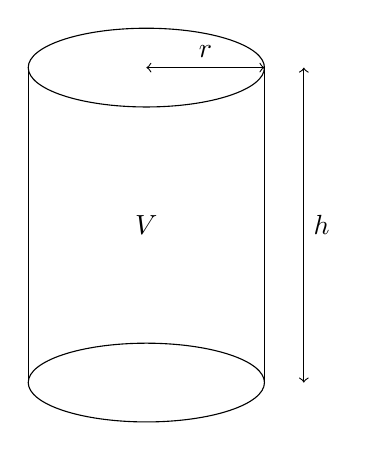
\begin{tikzpicture}
    % Cylinder
    \draw (0,0) ellipse (1.5cm and 0.5cm);
    \draw (0,4) ellipse (1.5cm and 0.5cm);
    \draw (-1.5,0) -- (-1.5,4);
    \draw (1.5,0) -- (1.5,4);
    
    % Labels
    \draw[<->] (2,0) -- (2,4) node[midway, right] {$h$};
    \draw[<->] (0,4) -- (1.5,4) node[midway, above] {$r$};
    \node at (0,2) {$V$};
\end{tikzpicture}
\end{center}
\end{problem}

\begin{hint}
Use the weighted AM-GM inequality where the weights correspond to the constraint structure.
\end{hint}

\begin{solution}
\textbf{(a) Proof:}
Consider the three positive numbers $p, p, q$. Applying AM-GM:
\begin{align*}
    \frac{p + p + q}{3} &\ge \sqrt[3]{p \cdot p \cdot q} \\
    \frac{2p + q}{3} &\ge \sqrt[3]{p^2 q} \\
    2p + q &\ge 3 \sqrt[3]{p^2 q}
\end{align*}

\textbf{(b) Application:}
Let Surface Area $A$ be constant, and we maximize Volume $V$.
\[ A = 2\pi r^2 + 2\pi rh \]
\[ V = \pi r^2 h \]
Split the curved surface area term $2\pi rh$ into two equal parts: $\pi rh$ and $\pi rh$.
Apply AM-GM to the three terms: $2\pi r^2$, $\pi rh$, and $\pi rh$.
\begin{align*}
    \text{Sum} &= 2\pi r^2 + \pi rh + \pi rh = A \quad (\text{Constant}) \\
    \text{Product} &= (2\pi r^2)(\pi rh)(\pi rh) = 2\pi^3 r^4 h^2 = 2\pi (\pi r^2 h)^2 = 2\pi V^2
\end{align*}
Using AM-GM:
\begin{align*}
    \frac{2\pi r^2 + \pi rh + \pi rh}{3} &\ge \sqrt[3]{2\pi V^2} \\
    \frac{A}{3} &\ge \sqrt[3]{2\pi V^2}
\end{align*}
Since $A$ is fixed, the maximum Volume $V$ occurs when equality holds.
Equality holds when the three terms are equal:
\begin{align*}
    2\pi r^2 &= \pi rh \\
    2r &= h
\end{align*}
Thus, the volume is maximized when the height equals the diameter. \hfill $\square$
\end{solution}

\begin{takeaways}
\begin{enumerate}
    \item \textbf{Weighted AM-GM:} When surface area terms have different coefficients, split larger terms to create equal weights in the AM-GM application.
    \item \textbf{Strategic Grouping:} Choose terms that when multiplied together yield a power of the volume expression to be maximized.
\end{enumerate}
\end{takeaways}


% Problem 9: Linear Growth Coefficients (Sample 04 - New)
% Problem 9: Pendulum Period and the AGM
\begin{problem}[Pendulum Motion and the AGM]

\noindent A simple pendulum of length $l$ is released from rest at the horizontal position ($\theta=\tfrac{\pi}{2}$). Let $\theta$ be the angle the pendulum makes with the downward vertical. From conservation of energy, the angular velocity satisfies:
\[
\left(\frac{d\theta}{dt}\right)^2=\frac{2g}{l}\cos\theta,
\]
where $g$ is the acceleration due to gravity. Let $T$ be the time taken for the pendulum 
to swing from the horizontal position ($\theta=\tfrac{\pi}{2}$) to the vertical position ($\theta=0$).
We can note that for small oscillations, $\cos\theta\approx1$, 
so $T \approx \sqrt{\frac{l}{2g}} \cdot \frac{\pi}{2}$. (Do NOT prove this approximation.)

\begin{enumerate}[label=(\roman*)]
    \item By using the substitution $\sin(\tfrac{\theta}{2}) = \tfrac{1}{\sqrt{2}}\sin\phi$, show that:
    \[
    T=\sqrt{\frac{l}{g}}\int_{0}^{\pi/2}\frac{d\phi}{\sqrt{1-\tfrac{1}{2}\sin^2\phi}}
    \]

    \item Let the elliptic-type integral
    \[
    I(a,b)=\int_0^{\pi/2}\frac{d\phi}{\sqrt{a^2\cos^2\phi+b^2\sin^2\phi}}.
    \]
    Show the expression for $T$ can be written as
    \[T=\sqrt{\frac{l}{g}}\,I\Bigl(1,\tfrac{1}{\sqrt2}\Bigr).\]

    \item Define sequences $a_1=1$, $b_1=\tfrac{1}{\sqrt2}$ and for $n\ge1$:
    \[a_{n+1}=\frac{a_n+b_n}{2},\qquad b_{n+1}=\sqrt{a_n b_n}.
    \]
    Show that $I(a_n,b_n)$ is invariant in $n$, and the sequences $a_n, b_n$ converge to the same limit. 
    Let $M=\lim_{n\to\infty} a_n=\lim_{n\to\infty} b_n$. 
    By taking limits show that the full period $P=4T$ satisfies
    \[P=\frac{2\pi\sqrt{l/g}}{M}.
    \]

    \item The small-angle (harmonic) approximation gives $P_0=2\pi\sqrt{l/g}$. Using $b_1<M<a_1$, deduce
    \[P_0 < P < \sqrt{2}\,P_0.
    \]
    Briefly explain why $P>P_0$.
\end{enumerate}

\end{problem}

\begin{hint}
\begin{itemize}
    \item For (i): Separate variables from the energy relation to get $dt$ in terms of $d\theta$, pick the correct sign for the motion, then substitute $\sin(\theta/2)=\tfrac{1}{\sqrt2}\sin\phi$ and change limits.
    \item For (ii): Use $\cos^2\phi+\sin^2\phi=1$ to rewrite the integrand into the form $a^2\cos^2\phi+b^2\sin^2\phi$.
    \item For (iii): Use the invariance to equate $I(1,1/\sqrt2)=I(M,M)$ and evaluate $I(M,M)=\pi/(2M)$.
    \item For (iv): Invert the inequalities to bound $1/M$, then multiply by $2\pi\sqrt{l/g}$; explain that large amplitude slows the motion compared to the small-angle linearisation.
\end{itemize}
\end{hint}

\begin{solution}

% Small illustrative pendulum diagram
\begin{center}
\begin{tikzpicture}[scale=1.0]
  % pivot O
  \coordinate (O) at (0,0);
  \coordinate (A) at (2,0); % vertical down position for reference
  % bob at horizontal start (theta = pi/2)
  \coordinate (B) at (0,-2);
  % draw support
  \draw (O) node[above] {$O$} -- (B) node[below] {$B$};
  \draw[dashed] (O) -- (A) node[right] {$\downarrow$};
  \draw (O) circle (0.03cm);
  \draw (0,0) -- ( -2,0 ) node[left] {$A$};
  % arc and angle label
  \draw[->] (-0.6,0) arc (180:270:0.6) node[midway,left] {$\theta$};
  % length label
  \draw[<->] (0,-2.2) -- (0,0.15) node[midway,right] {$l$};
\end{tikzpicture}
\end{center}

\textbf{(i)} From energy, $d\theta/dt=-\sqrt{(2g/l)\cos\theta}$ for the downward swing. Thus
\[T=\sqrt{\tfrac{l}{2g}}\int_0^{\pi/2}\frac{d\theta}{\sqrt{\cos\theta}}.
\]
With $\sin(\theta/2)=\tfrac{1}{\sqrt2}\sin\phi$ one finds $\cos\theta=\cos^2\phi$ and
\[d\theta=\frac{\sqrt{2}\cos\phi}{\sqrt{1-\tfrac{1}{2}\sin^2\phi}}\,d\phi,
\]
which yields the stated integral.

\textbf{(ii)} Note $1-\tfrac{1}{2}\sin^2\phi=\cos^2\phi+\tfrac{1}{2}\sin^2\phi$, so the integrand is of the form in $I(a,b)$ with $a=1$, $b=1/\sqrt2$.

\textbf{(iii)} By invariance $I(1,1/\sqrt2)=I(M,M)=\int_0^{\pi/2}d\phi/(M)=\pi/(2M)$. Hence
\[T=\sqrt{\tfrac{l}{g}}\cdot\frac{\pi}{2M},\qquad P=4T=\frac{2\pi\sqrt{l/g}}{M}.
\]

\textbf{(iv)} Since $b_1< M< a_1$ we have $1/\sqrt2< M<1$, so $1<1/M<\sqrt2$. Multiplying by $2\pi\sqrt{l/g}$ gives $P_0<P<\sqrt2\,P_0$. Physically, for large amplitude the restoring tangential acceleration is not proportional to $\theta$, so the motion is slower than the small-angle linear approximation.
\end{solution}

\begin{takeaways}
\begin{enumerate}
    \item The pendulum period for large amplitude leads to elliptic integrals; the AGM gives an efficient exact representation.
    \item Recursive arithmetic–geometric mean sequences converge rapidly and can be used to evaluate certain definite integrals.
    \item Small-angle linearisation underestimates the true period; inequalities give sharp bounds on the error.
\end{enumerate}
\end{takeaways}



\begin{problem}[Linear Growth Coefficients]
Let \(P(z)=a_n z^n + a_{n-1} z^{n-1}+\dots+a_1 z\) be a polynomial with complex coefficients satisfying
\(|a_k|\le k\) for all $1\le k\le n$.

\begin{enumerate}[label=(\roman*)]
    \item Show that for real $x$ with $|x|<1$:
    \[\sum_{k=1}^\infty k x^k = \frac{x}{(1-x)^2}.
    \]
    \item Using (i), prove that for $|z|<1$:
    \[|P(z)| < \frac{|z|}{(1-|z|)^2}.
    \]
    \item Deduce that if $P(z)=1$ and $|z|<1$ then
    \[|z|>\frac{3-\sqrt{5}}{2}.
    \]
    \item If instead $Q(z)=b_n z^n+\dots+b_1 z$ with $|b_k|\le1$, show any root of $Q(z)=1$ with $|z|<1$ satisfies $|z|>\tfrac12$.
\end{enumerate}
\end{problem}

\begin{hint}
Differentiate the geometric series to obtain (i). For (ii) apply the triangle inequality and compare the finite sum with the infinite series from (i). For (iii) set $r=|z|$ and solve the inequality $1<r/(1-r)^2$. For (iv) repeat with the bound $|b_k|\le1$ and the standard geometric series.
\end{hint}

\begin{solution}
	\textbf{(i)} Differentiate $\sum_{k=0}^\infty x^k=1/(1-x)$ (valid for $|x|<1$) to get
\[\sum_{k=1}^\infty k x^{k-1}=\frac{1}{(1-x)^2},\]
then multiply by $x$ to obtain the stated formula.

	\textbf{(ii)} For $|z|<1$ the triangle inequality gives
\[|P(z)|\le\sum_{k=1}^n |a_k||z|^k\le\sum_{k=1}^n k|z|^k<\sum_{k=1}^\infty k|z|^k=\frac{|z|}{(1-|z|)^2}.
\]

	\textbf{(iii)} If $P(z)=1$ then $1<\dfrac{r}{(1-r)^2}$ with $r=|z|$. Rearranging yields
\[r^2-3r+1<0,
\]
whose roots are $(3\pm\sqrt{5})/2$. Since $r<1$ we obtain $r>\dfrac{3-\sqrt{5}}{2}$.

	\textbf{(iv)} With $|b_k|\le1$ we have
\[1=|Q(z)|\le\sum_{k=1}^n |z|^k<\sum_{k=1}^\infty r^k=\frac{r}{1-r},
\]
so $1<r/(1-r)$, giving $r>1/2$.
\end{solution}

\begin{takeaways}
\begin{enumerate}
    \item Differentiate power series to obtain weighted sums like $\sum kx^k$.
    \item Bounding $|P(z)|$ by a real series is a reliable method to locate roots in the complex plane.
    \item Coefficient growth affects how close roots can lie to the origin: larger coefficients allow roots nearer $0$.
\end{enumerate}
\end{takeaways}

% Problem 2: Tetrahedron Volume (Sample 03)
\begin{problem}[Cauchy-Schwarz and Plane Intersections]
(a) Let $x, y, z$ be positive real numbers. Prove that:
\[ (x + y + z)\left(\frac{1}{x} + \frac{1}{y} + \frac{1}{z}\right) \ge 9 \]

(b) A plane passes through the fixed point $P(a, b, c)$ where $a,b,c > 0$. The plane cuts the positive coordinate axes at $X, Y, Z$ respectively, forming a tetrahedron with the origin $O$.
Show that the minimum volume of the tetrahedron $OXYZ$ is $\frac{9}{2}abc$.

\vspace{1cm}

\begin{center}
% Slightly rotated 3D projection and hidden edges styled
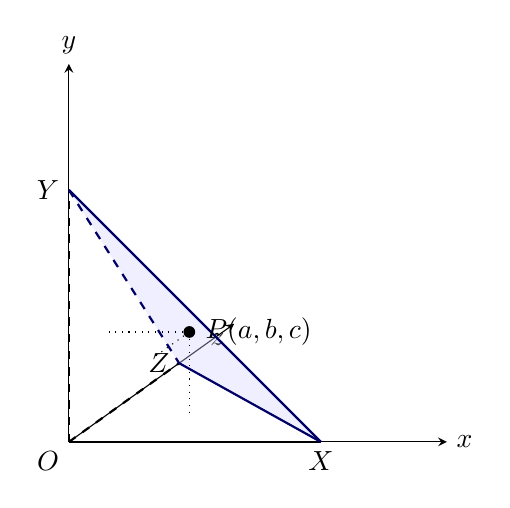
\begin{tikzpicture}[
    x={(0.8cm,0cm)},
    y={(0cm,0.8cm)},
    z={(0.35cm,0.25cm)},
    >=stealth]
    % Axes (tilted for better perspective)
    \draw[->] (0,0,0) -- (6,0,0) node[right] {$x$};
    \draw[->] (0,0,0) -- (0,6,0) node[above] {$y$};
    \draw[->] (0,0,0) -- (0,0,6) node[below left] {$z$};

    % Plane Intercepts
    \coordinate (X) at (4,0,0);
    \coordinate (Y) at (0,4,0);
    \coordinate (Z) at (0,0,4);

    % Tetrahedron edges from origin
    \draw[thick] (0,0,0) -- (X);
    \draw[thick,dashed] (0,0,0) -- (Y); % hidden
    \draw[thick,dashed] (0,0,0) -- (Z); % hidden

    % Draw Plane triangle XYZ (tweaked color/opacity)
    \fill[blue!18, opacity=0.35] (X) -- (Y) -- (Z) -- cycle;
    % Visible edges
    \draw[thick, blue!40!black] (X) -- (Y);
    \draw[thick, blue!40!black] (X) -- (Z);
    % Edge potentially behind (style as dashed)
    \draw[thick,dashed, blue!40!black] (Y) -- (Z);

    % Point P (projected inside)
    \node[circle, fill, inner sep=1.5pt, label=right:{$P(a,b,c)$}] at (1.33, 1.33, 1.33) {};

    % Helper dotted projections from P to axes/intercepts (optional visibility cues)
    \draw[dotted] (1.33,1.33,1.33) -- (1.33,1.33,0);
    \draw[dotted] (1.33,1.33,1.33) -- (1.33,0,1.33);
    \draw[dotted] (1.33,1.33,1.33) -- (0,1.33,1.33);

    % Labels
    \node[below] at (X) {$X$};
    \node[left] at (Y) {$Y$};
    \node[left] at (Z) {$Z$};
    \node[below left] at (0,0,0) {$O$};
\end{tikzpicture}
\end{center}
\end{problem}

\begin{hint}
Apply Cauchy-Schwarz to vectors formed by coordinates and reciprocals. The volume formula involves the product of intercepts.
\end{hint}

\begin{solution}
\textbf{(a) Proof:}
Apply AM-GM to the sums separately.

1. $(x+y+z) \ge 3\sqrt[3]{xyz}$

2. $(\frac{1}{x} + \frac{1}{y} + \frac{1}{z}) \ge 3\sqrt[3]{\frac{1}{xyz}}$

Multiplying the inequalities (since all terms are positive):

\[ (x+y+z)\left(\frac{1}{x} + \frac{1}{y} + \frac{1}{z}\right) \ge \left(3\sqrt[3]{xyz}\right) \left(\frac{3}{\sqrt[3]{xyz}}\right) = 9 \]

\textbf{(b) Application:}
Let the intercepts be $X(x_0, 0, 0)$, $Y(0, y_0, 0)$, and $Z(0, 0, z_0)$.
The equation of the plane is:
\[ \frac{x}{x_0} + \frac{y}{y_0} + \frac{z}{z_0} = 1 \]
Since the plane passes through $P(a,b,c)$:
\[ \frac{a}{x_0} + \frac{b}{y_0} + \frac{c}{z_0} = 1 \]
The Volume of the tetrahedron is $V = \frac{1}{6} x_0 y_0 z_0$. We want to minimize this product.
Apply AM-GM to the three terms summing to 1:
\begin{align*}
    \frac{\frac{a}{x_0} + \frac{b}{y_0} + \frac{c}{z_0}}{3} &\ge \sqrt[3]{\frac{abc}{x_0 y_0 z_0}} \\
    \frac{1}{3} &\ge \sqrt[3]{\frac{abc}{6V}} \quad (\text{Since } x_0 y_0 z_0 = 6V)
\end{align*}
Cube both sides:
\begin{align*}
    \frac{1}{27} &\ge \frac{abc}{6V} \\
    6V &\ge 27abc \\
    V &\ge \frac{9}{2}abc
\end{align*}
Thus, the minimum volume is $\frac{9}{2}abc$. \hfill $\square$
\end{solution}

\begin{takeaways}
\begin{enumerate}
    \item \textbf{Multiplying Inequalities:} When all terms are positive, inequalities can be multiplied directly to achieve stronger bounds.
    \item \textbf{Constraint Optimization:} Use the constraint equation to express the objective function, then apply AM-GM to the constraint terms.
\end{enumerate}
\end{takeaways}

\begin{remark}[Alternate proof for part (a)]
By Cauchy--Schwarz,
\[
    (x+y+z)\Big(\tfrac{1}{x}+\tfrac{1}{y}+\tfrac{1}{z}\Big)
    \ge (1+1+1)^2 = 9,
\]
with equality at $x=y=z$. This gives the same bound in one step.
\end{remark}

% Problem 3: Sphere Inscriptions (Sample 04)
\begin{problem}[Cube in Sphere Optimization]
(a) Establish the inequality $u^2 + v^2 + w^2 \ge 3(uvw)^{\frac{2}{3}}$ for positive numbers $u, v, w$.

(b) A rectangular prism is inscribed inside a sphere of fixed radius $R$.
Show that the prism has the maximum volume when it is a cube.

\vspace{1cm}

\begin{center}
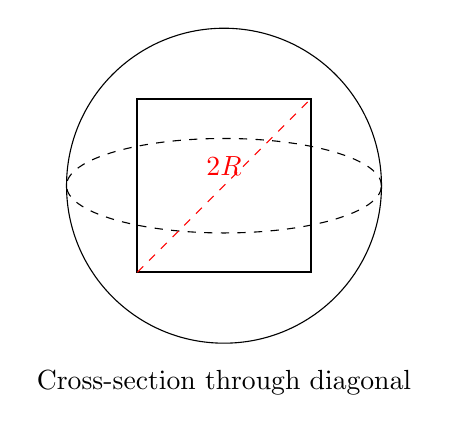
\begin{tikzpicture}
    % Sphere
    \draw (0,0) circle (2cm);
    \draw[dashed] (0,0) ellipse (2cm and 0.6cm);
    
    % Inscribed Rectangular approximation (2D projection)
    \draw[thick] (-1.1,-1.1) rectangle (1.1,1.1);
    
    % Diagonal
    \draw[dashed, red] (-1.1,-1.1) -- (1.1,1.1);
    \node[red, above] at (0,0) {$2R$};
    
    % Label
    \node at (0, -2.5) {Cross-section through diagonal};
\end{tikzpicture}
\end{center}
\end{problem}

\begin{hint}
Establish the relationship between edge length and sphere radius, then apply AM-GM to the constraint.
\end{hint}

\begin{solution}
\textbf{(a) Proof:}
Let the three terms be $u^2, v^2, w^2$. Applying AM-GM:
\begin{align*}
    \frac{u^2 + v^2 + w^2}{3} &\ge \sqrt[3]{u^2 v^2 w^2} \\
    u^2 + v^2 + w^2 &\ge 3 (uvw)^{2/3}
\end{align*}

\textbf{(b) Application:}
Let the dimensions of the prism be $x, y, z$.
The prism is inscribed in a sphere of radius $R$, meaning the space diagonal of the prism equals the diameter of the sphere ($2R$).
\[ x^2 + y^2 + z^2 = (2R)^2 = 4R^2 \quad (\text{Constant}) \]
We wish to maximize the Volume $V = xyz$.
Substitute $u=x, v=y, w=z$ into the inequality from part (a):
\begin{align*}
    x^2 + y^2 + z^2 &\ge 3 (xyz)^{2/3} \\
    4R^2 &\ge 3 V^{2/3}
\end{align*}
Rearranging for $V$:
\begin{align*}
    \frac{4R^2}{3} &\ge V^{2/3} \\
    \left(\frac{4R^2}{3}\right)^{3/2} &\ge V
\end{align*}
The Volume $V$ is bounded by a constant. The maximum occurs when equality holds in the AM-GM step.
Equality requires:
\[ x^2 = y^2 = z^2 \implies x = y = z \]
Therefore, the rectangular prism must be a cube to maximize the volume. \hfill $\square$
\end{solution}

\begin{takeaways}
\begin{enumerate}
    \item \textbf{Constraint Transformation:} Convert geometric constraints (sphere inscribed in cube) into algebraic relationships between variables.
    \item \textbf{Substitution Strategy:} Identify which form of AM-GM to use based on the powers appearing in your objective function.
\end{enumerate}
\end{takeaways}

% Problem 4: Complex Series Summation (Sample 43)
\begin{problem}[De Moivre's Theorem and Geometric Series]
Let $\alpha = \cos\theta + i \sin\theta$ and consider the series 

\[ 
C = \alpha^{-n} + \alpha^{-n+1} + \dots + \alpha^{-1} + \alpha^0 + \alpha^1 + \dots + \alpha^n 
\] for a positive integer $n$.

\begin{enumerate}[label=(\roman*)]
    \item Show that $\alpha^k + \alpha^{-k} = 2 \cos k\theta$.
    \item Prove that 
    
    \[
    C = \frac{\alpha^n + \alpha^{-n} - (\alpha^{n+1} + \alpha^{-(n+1)})}{(1-\alpha)(1-\bar{\alpha})}
    \]
    where $\bar{\alpha}$ is the complex conjugate of $\alpha$.

    \item Deduce that 
    
    \[
    1 + 2\sum_{k=1}^n \cos k\theta 
    = \frac{\cos n\theta - \cos (n+1)\theta}{1 - \cos\theta}.
    \]

    \item Show that 
    
    \[ 
    \sum_{k=1}^n \cos \frac{k\pi}{n} = -1 \quad \text{(independent of $n$)}.
    \]
\end{enumerate}
\end{problem}

\begin{hint}
Use De Moivre's theorem to express $\sin(n\theta)$ in terms of $z = e^{i\theta}$, then sum the resulting geometric series.
\end{hint}

\begin{solution}
\begin{enumerate}[label=(\roman*)]
    \item Since $\alpha = \cos\theta + i \sin\theta$, by De Moivre's Theorem:
    $$\alpha^k = \cos k\theta + i \sin k\theta, \quad \alpha^{-k} = \cos k\theta - i \sin k\theta$$
    Adding: $\alpha^k + \alpha^{-k} = 2 \cos k\theta$.

    \item The series $C$ is geometric with first term $\alpha^{-n}$, ratio $\alpha$, and $(2n+1)$ terms:
    $$C = \frac{\alpha^{-n}(\alpha^{2n+1} - 1)}{\alpha - 1} = \frac{\alpha^{n+1} - \alpha^{-n}}{\alpha - 1}$$
    Multiply by $\frac{\bar{\alpha} - 1}{\bar{\alpha} - 1}$:
    $$C = \frac{(\alpha^{n+1} - \alpha^{-n})(\bar{\alpha} - 1)}{(\alpha - 1)(\bar{\alpha} - 1)}$$
    Since $(\alpha - 1)(\bar{\alpha} - 1) = 2(1-\cos\theta)$ and expanding the numerator:
    $$C = \frac{\alpha^n + \alpha^{-n} - (\alpha^{n+1} + \alpha^{-(n+1)})}{(1-\alpha)(1-\bar{\alpha})}$$

    \item From the definition: $C = 1 + \sum_{k=1}^n (\alpha^k + \alpha^{-k}) = 1 + 2\sum_{k=1}^n \cos k\theta$
    Using part (ii) with $\alpha^k + \alpha^{-k} = 2\cos k\theta$:
    $$1 + 2\sum_{k=1}^n \cos k\theta = \frac{\cos n\theta - \cos (n+1)\theta}{1 - \cos\theta}$$

    \item Substitute $\theta = \frac{\pi}{n}$:
    $$1 + 2\sum_{k=1}^n \cos \frac{k\pi}{n} = \frac{\cos \pi - \cos \left(\pi + \frac{\pi}{n}\right)}{1 - \cos \frac{\pi}{n}}$$
    Since $\cos\pi = -1$ and $\cos(\pi + x) = -\cos x$:
    $$1 + 2\sum_{k=1}^n \cos \frac{k\pi}{n} = \frac{-1 + \cos \frac{\pi}{n}}{1 - \cos \frac{\pi}{n}} = -1$$
    Therefore: $\sum_{k=1}^n \cos \frac{k\pi}{n} = -1$.
\end{enumerate}
\end{solution}

\begin{takeaways}
\begin{enumerate}
    \item \textbf{Geometric Series with Complex Numbers:} Apply standard formulas but manipulate using conjugates when needed.
    \item \textbf{Trigonometric Identities:} De Moivre's theorem connects complex exponentials to trigonometric sums.
\end{enumerate}
\end{takeaways}

% Problem 5: Orthogonality and Roots of Unity (Sample 60)
\begin{problem}[Complex Number Perpendicularity]
Let $n$ be a positive integer, and let $z_k = e^{i\frac{2k\pi}{n}}$ for $k \in \{1, 2, \dots, n\}$.

Let $z_a, z_b,$ and $z_c$ be three distinct complex numbers from this set. Prove that if they satisfy the equation:
\[
\frac{z_a}{z_b} = - \frac{z_c}{z_a}
\]
then the vector represented by the sum $z_b + z_c$ is perpendicular to the vector $z_a$.
\end{problem}

\begin{hint}
\begin{enumerate}
    \item Use the given equation to express $\frac{z_c}{z_a}$ in terms of $\frac{z_b}{z_a}$.
    \item Recall that two complex numbers $w_1$ and $w_2$ are perpendicular if their ratio $\frac{w_1}{w_2}$ is purely imaginary.
    \item Form the ratio $Z = \frac{z_b + z_c}{z_a}$ and simplify using the given condition.
    \item For any complex number $u$ on the unit circle, $u - \frac{1}{u} = u - \overline{u} = 2i\text{Im}(u)$ is purely imaginary.
\end{enumerate}
\end{hint}

\begin{solution}
To prove perpendicularity, we show that $Z = \frac{z_b + z_c}{z_a}$ is purely imaginary.

\textbf{Step 1:} Express the ratio:
\[
Z = \frac{z_b + z_c}{z_a} = \frac{z_b}{z_a} + \frac{z_c}{z_a}
\]

\textbf{Step 2:} From the given condition $\frac{z_a}{z_b} = -\frac{z_c}{z_a}$, rearrange:
\[
\frac{z_c}{z_a} = -\frac{z_a}{z_b}
\]

\textbf{Step 3:} Substitute into $Z$:
\[
Z = \frac{z_b}{z_a} - \frac{z_a}{z_b}
\]

\textbf{Step 4:} Let $u = \frac{z_b}{z_a}$. Since both $z_a$ and $z_b$ are roots of unity, $|u|=1$, so $\overline{u} = \frac{1}{u}$.
\[
Z = u - \frac{1}{u} = u - \overline{u} = 2i \cdot \text{Im}(u)
\]

Since $Z$ is purely imaginary, the vectors $z_b + z_c$ and $z_a$ are perpendicular.
\end{solution}

\begin{takeaways}
\begin{enumerate}
    \item \textbf{Perpendicularity Test:} For complex numbers, perpendicularity is equivalent to having a purely imaginary ratio.
    \item \textbf{Unit Circle Property:} When $|z|=1$, we have $\overline{z} = \frac{1}{z}$, which simplifies many algebraic manipulations.
    \item \textbf{Conjugate Differences:} The expression $z - \overline{z}$ is always purely imaginary, while $z + \overline{z}$ is purely real.
\end{enumerate}
\end{takeaways}

% Additional medium problems from the selection would continue here...
% (Samples 07, 09, 10, 12, 15, 17, 18, 21, 28, 30, 35, 36, 55)

% Problem 6: Sequence of Rectangles (Sample 05)
\begin{problem}[Converging Rectangles — Newton's Method for $\sqrt{2}$]
Consider a sequence of rectangles with side lengths $a_n$ and $b_n$. The first rectangle has $a_1=2$ and $b_1=1$. For integers $n\ge1$ define
\[
a_{n+1}=\frac{a_n+b_n}{2},\qquad b_{n+1}=\frac{2}{a_{n+1}}.
\]

\begin{enumerate}[label=(\roman*)]
    \item Show that every rectangle in the sequence has area $2$.
    \item Prove that $a_n\ge\sqrt{2}$ for all $n\ge1$.
    \item Show by induction that
    \[a_n-\sqrt{2}\le\frac{1}{2^{n-1}}(2-\sqrt{2}),\qquad n\ge1.
    \]
    \item Deduce that the rectangles approach a square as $n\to\infty$.
    \item (Optional, no points) Use a calculator to find the first five terms of the sequence $a_n$ and comment on the speed of convergence to the actual value of $\sqrt{2}$.
\end{enumerate}
\end{problem}

\begin{hint}
For (i) compute $A_{n+1}=a_{n+1}b_{n+1}$ directly. For (ii) apply AM--GM to $a_n$ and $b_n$ and use the area from (i). For (iii) express $a_{k+1}-\sqrt2$ in terms of $(a_k-\sqrt2)^2$ and bound the multiplicative factor by $\tfrac12$. For (iv) use the squeeze theorem together with the bound in (iii).
\end{hint}

\begin{solution}
	\textbf{(i)} The area is $A_n=a_n b_n$. Using the recursion,
\[A_{n+1}=a_{n+1}b_{n+1}=a_{n+1}\cdot\frac{2}{a_{n+1}}=2,
\]
so $A_n\equiv2$ for all $n$.

	\textbf{(ii)} By AM--GM,
\[a_{n+1}=\frac{a_n+b_n}{2}\ge\sqrt{a_n b_n}=\sqrt{2},\]
and the base case $a_1=2\ge\sqrt2$ holds, so $a_n\ge\sqrt2$ for all $n$.

	\textbf{(iii)} From $b_k=2/a_k$ we get
\[a_{k+1}=\frac{a_k+\frac{2}{a_k}}{2}=\frac{a_k^2+2}{2a_k}.
\]
Subtracting $\sqrt2$ and simplifying yields
\[a_{k+1}-\sqrt2=\frac{(a_k-\sqrt2)^2}{2a_k}.
\]
Since $a_k\ge\sqrt2$, the factor $1/(2a_k)\le 1/(2\sqrt2)<\tfrac12$, hence
\[a_{k+1}-\sqrt2\le \tfrac12 (a_k-\sqrt2).
\]
Applying the inductive hypothesis gives the claimed bound.

	\textbf{(iv)} From (ii) and (iii) we have
\[0\le a_n-\sqrt2\le\frac{2-\sqrt2}{2^{n-1}}\to0\quad(n\to\infty).
\]
Since $a_n b_n=2$ for all $n$, it follows $b_n\to\sqrt2$ as well. Therefore the side lengths both tend to $\sqrt2$ and the rectangles approach a square.
\end{solution}

\begin{takeaways}
\begin{enumerate}
    % \item Simple recurrences combined with AM--GM often give quick monotonicity or lower/upper bounds.
    % \item Expressing the next error term as a square of the previous error (as in part (iii)) gives fast geometric decay.
    % \item The squeeze theorem is a convenient final step to convert explicit bounds into limits.
    \item Newton's Method: This problem is actually a geometric visualization of Newton's Method 
    for estimating square roots. 
    The recurrence $a_{n+1} = \frac{1}{2}(a_n + \frac{2}{a_n})$ 
    is the standard algorithm for calculating $\sqrt{2}$.
    \item Convergence Speed: While the problem asks to prove linear convergence (error halves each time), 
    Newton's method actually converges quadratically 
    (the number of correct digits doubles with every step), 
    which is much faster than the bound proven in part (iii).

    \item AM-GM Utility: The arithmetic mean of a number and its reciprocal (scaled) 
    is a classic way to generate a value closer to the root, 
    bounded below by the root itself.
\end{enumerate}
\end{takeaways}


% \usepackage{booktabs}
% \usepackage{amsmath}
% \usepackage{geometry}
\begin{table}[h!]
\centering
\caption{Convergence of sequence $a_n$ to $\sqrt{2}$ (Newton's Method)}
\label{tab:newton_convergence}
\renewcommand{\arraystretch}{1.2}
\begin{tabular}{@{}c l l l c@{}}
% \toprule
\textbf{n} & \textbf{Exact Fraction ($a_n$)} & \textbf{Decimal Approx.} & \textbf{Error ($|a_n - \sqrt{2}|$)} & \textbf{Correct Digits} \\
% \midrule
1 & $2$ & $2.0000000000$ & $5.86 \times 10^{-1}$ & 1 \\
2 & $\frac{3}{2}$ & $1.5000000000$ & $8.58 \times 10^{-2}$ & 1 \\
3 & $\frac{17}{12}$ & $1.4166666667$ & $2.45 \times 10^{-3}$ & 3 \\
4 & $\frac{577}{408}$ & $1.4142156863$ & $2.12 \times 10^{-6}$ & 6 \\
5 & $\frac{665857}{470832}$ & $1.4142135624$ & $1.59 \times 10^{-12}$ & 12 \\
6 & $\frac{886731088897}{627013566048}$ & $1.4142135623$ & $8.86 \times 10^{-25}$ & 24 \\
7 & (too large to display) & $1.4142135623$ & $2.75 \times 10^{-49}$ & 49 \\
8 & (too large to display) & $1.4142135623$ & $2.64 \times 10^{-98}$ & 98 \\
9 & (too large to display) & $1.4142135623$ & $2.44 \times 10^{-196}$ & 196 \\
10 & (too large to display) & $1.4142135623$ & $2.08 \times 10^{-392}$ & 392 \\
% \bottomrule
\end{tabular}

\vspace{0.3cm}
\small \textbf{Performance Evaluation:} The sequence exhibits \textit{Quadratic Convergence}, meaning the number of correct digits roughly doubles with every iteration. By $n=10$, the value is accurate to nearly 400 decimal places.
\end{table}

% Problem 7: Integrals and Combinatorial Identity (Sample 06)
\begin{problem}[Integrals and a Combinatorial Identity]\label{prob:part2-integral-identity-06}
Let $I_n$ be defined for integers $n\ge0$ by
\[
I_n=\int_{-1}^0 x^n\sqrt{x+1}\,dx.
\]
\begin{enumerate}[label=(\roman*)]
    \item Use integration by parts to show that, for $n\ge1$,
    \[I_n=\frac{-2n}{2n+3}\,I_{n-1}.
    \]
    \item Hence prove
    \[I_n = (-1)^n\frac{2^{n+1}n!}{3\times5\times\dots\times(2n+3)}.
    \]
    \item By substituting $u=\sqrt{x+1}$, show that
    \[I_n = 2\sum_{k=0}^n (-1)^{n-k}\binom{n}{k}\frac{1}{2k+3}.
    \]
    \item Deduce the combinatorial identity
    \[\sum_{k=0}^n (-1)^k \binom{n}{k}\frac{1}{2k+3} = \frac{2^n n!}{3\times5\times\dots\times(2n+3)}.
    \]
\end{enumerate}
\end{problem}

\begin{hint}
For (i) take $u=x^n$ and $dv=(x+1)^{1/2}dx$ and use $x=(x+1)-1$ to relate $I_n$ and $I_{n-1}$. 

For (ii) evaluate $I_0$ and iterate the reduction. 

For (iii) substitute $u=\sqrt{x+1}$ so $x=u^2-1$ and expand by the binomial theorem before integrating. 

For (iv) equate the two expressions for $I_n$ and simplify.

\end{hint}

\begin{solution}
	\textbf{(i)} Integration by parts with $u=x^n$, $v=\tfrac{2}{3}(x+1)^{3/2}$ yields after rearrangement
\[I_n=\frac{-2n}{2n+3}I_{n-1}.
\]

	\textbf{(ii)} $I_0=\int_{-1}^0 (x+1)^{1/2}dx=\tfrac{2}{3}$. Repeated application of the reduction gives the stated closed form.
	
    \[ I_n = \left( \frac{-2n}{2n+3} \right) \left( \frac{-2(n-1)}{2n+1} \right) \dots \left( \frac{-2(1)}{5} \right) I_0
    \]

    \[ I_n = (-1)^n \frac{2^n n!}{(2n+3)(2n+1)\dots(5)} \cdot \frac{2}{3} = (-1)^n \frac{2^{n+1} n!}{3 \times 5 \times \dots \times (2n+3)}
    \]

    \textbf{(iii)} With $u=\sqrt{x+1}$ we have $dx=2u\,du$, $x=u^2-1$ 
    and using the binomial theorem,

    \[u^2(u^2-1)^n = \sum_{k=0}^n (-1)^{n-k}\binom{n}{k}u^{2k+2}.
    \]

    hence

    \[I_n=2\int_0^1 u^2(u^2-1)^n\,du=2\sum_{k=0}^n (-1)^{n-k}\binom{n}{k}\frac{1}{2k+3}.
    \]

	\textbf{(iv)} Equating the expressions in (ii) and (iii) and cancelling $2(-1)^n$ yields the required identity.
\end{solution}

\begin{takeaways}
\begin{enumerate}
    \item \textbf{The Power of Two Methods:} Reduction formulas and substitutions give two complementary approaches to definite integrals; equating them often produces useful combinatorial identities.
    % \item Familiarity with double-factorial-like products (odd products) is useful when working with reduction formulas arising from square-root weights.
    % \item \textbf{Double Factorials:} This problem reinforces familiarity with products of odd integers ($3 \times 5 \times \dots$), a common pattern in reduction formulas involving square roots.
    \item \textbf{Algebraic Manipulation:} The trick in step (i) of splitting $(x+1)$ to recover $I_n + I_{n-1}$ is a recurring motif in Extension 2 integration problems.
    \item \textbf{Double Factorial:} It is often helpful to express products of integers using double factorial notation to simplify expressions and recognize patterns.
    
    For odd numbers, $(2n+1)!! = 1 \times 3 \times 5 \times \dots \times (2n+1) = \frac{(2n+1)!}{2^n n!}$.

    For even numbers, $(2n)!! = 2 \times 4 \times 6 \times \dots \times (2n) = 2^n n!$.

    And we can write the equation in a beautifully compact form:
    
      \[\sum_{k=0}^n (-1)^k \binom{n}{k}\frac{1}{2k+3} 
      = \frac{(2n)!!}{(2n+3)!!}.
    \]
\end{enumerate}
\end{takeaways}